\begin{frameb}{w}{Images/Coma.jpg}
	\frametitle{Dark Matter}
	\framesubtitle{The Problem}
\end{frameb}

\begin{frameb}{w}{Images/NGC.jpg}
	\frametitle{Dark Matter}
	\framesubtitle{The Problem}
\end{frameb}

\begin{frame}
	\frametitle{Dark Matter}
	\framesubtitle{The Problem}

	\begin{columns}
	\begin{column}{0.5\textwidth}
		\begin{itemize}
			\item<1-> Observed by Fritz Zwicky in 1933.
			\item<2-> There appears to be a large amount of matter which we cannot see.
			\item<3-> Outnumbers traditional matter 7:1
		\end{itemize}
	\end{column}
	\begin{column}{0.5\textwidth}
		~ ~ ~\includegraphics<1->[width=\textwidth]{Images/zwicky.jpg}	
	\end{column}
	\end{columns}
\end{frame}


\begin{frame}
  \frametitle{What actually is Dark Matter?}
  \begin{itemize}
    \item<1-> Short answer: \only<2->{We don't know!}
    \item<3-> MACHOs: Massive Compact Halo Object
    \item<5-> WIMPs : Weakly Interacting Massive Particles
    \item<7-> Much effort has been put into trying to find the ``missing matter'' -but so far to no avail.
    \item<8-> Right now it's really just a name for a phenomenon we don't understand yet.
  \end{itemize}
  \onslide<4->{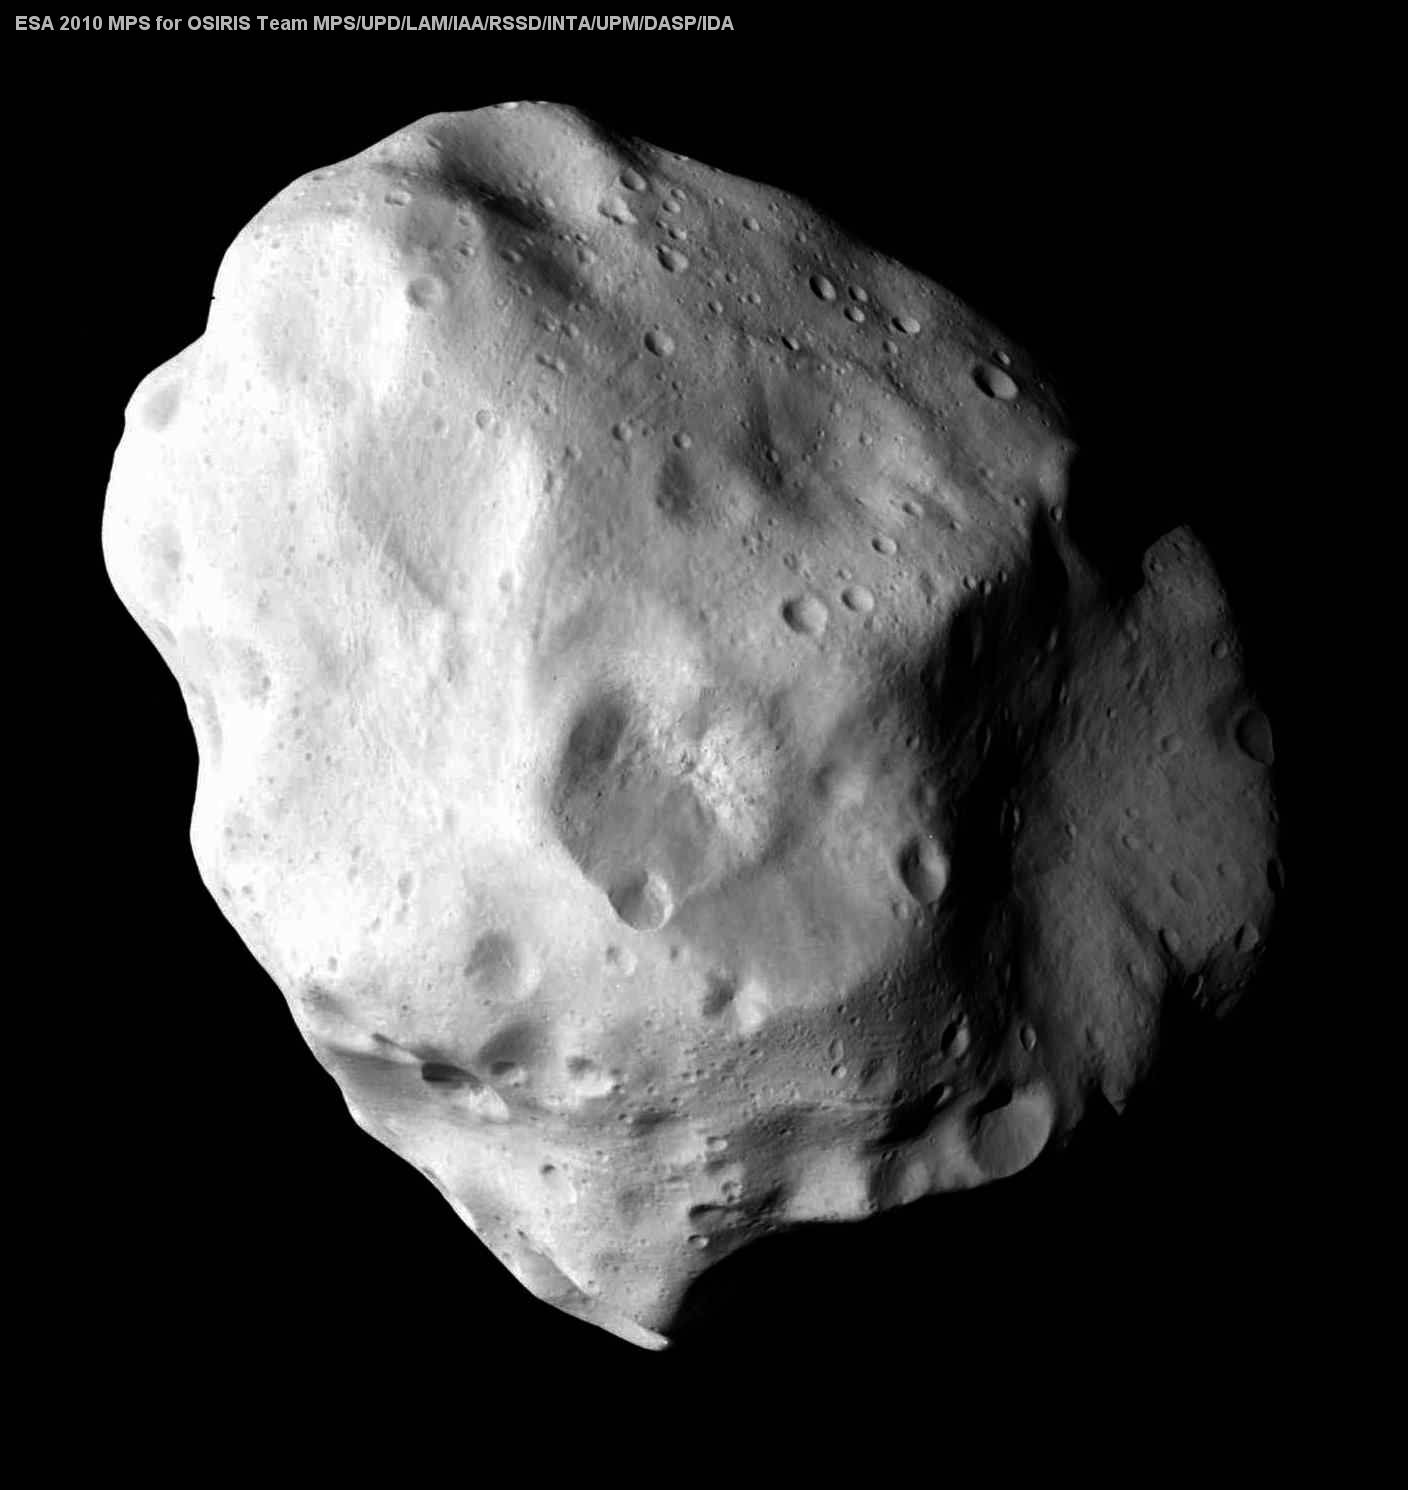
\includegraphics[height=0.4\textheight]{Images/asteroid.jpg}}
  \hspace{10pt}
  \onslide<6->{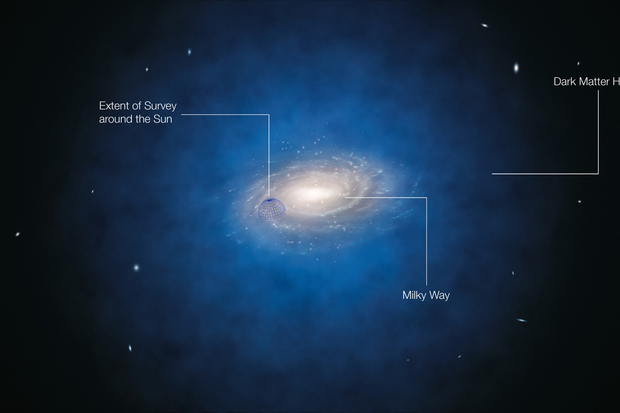
\includegraphics[height=0.4\textheight]{Images/wimp.jpg}}
\end{frame}

